\let\negmedspace\undefined
\let\negthickspace\undefined
\documentclass[journal]{IEEEtran}
\usepackage[a5paper, margin=10mm, onecolumn]{geometry}
%\usepackage{lmodern} % Ensure lmodern is loaded for pdflatex
\usepackage{tfrupee} % Include tfrupee package

\setlength{\headheight}{1cm} % Set the height of the header box
\setlength{\headsep}{0mm}     % Set the distance between the header box and the top of the text

\usepackage{gvv-book}
\usepackage{gvv}
\usepackage{cite}
\usepackage{amsmath,amssymb,amsfonts,amsthm}
\usepackage{algorithmic}
\usepackage{graphicx}
\usepackage{textcomp}
\usepackage{xcolor}
\usepackage{txfonts}
\usepackage{listings}
\usepackage{enumitem}
\usepackage{mathtools}
\usepackage{gensymb}
\usepackage{comment}
\usepackage[breaklinks=true]{hyperref}
\usepackage{tkz-euclide} 
\usepackage{listings}
% \usepackage{gvv}                                        
\def\inputGnumericTable{}                                 
\usepackage[latin1]{inputenc}                                
\usepackage{color}                                            
\usepackage{array}                                            
\usepackage{longtable}                                       
\usepackage{calc}                                             
\usepackage{multirow}                                         
\usepackage{hhline}                                           
\usepackage{ifthen}                                           
\usepackage{lscape}

\begin{document}

\bibliographystyle{IEEEtran}
\vspace{3cm}

\title{5.8.13}
\author{EE25BTECH11015 - Bhoomika V}
% \maketitle
% \newpage
% \bigskip
{\let\newpage\relax\maketitle}

\renewcommand{\thefigure}{\theenumi}
\renewcommand{\thetable}{\theenumi}
\setlength{\intextsep}{10pt} % Space between text and floats


\numberwithin{equation}{enumi}
\numberwithin{figure}{enumi}
\renewcommand{\thetable}{\theenumi}
\parindent 0px 
{Question :-} \\ 
The difference between two numbers is 26 and one number is three times the other. Find them.\\ 
\solution \\
Let the two numbers be $x$ and $y$ ($x > y$).

 Define equations
From the problem:

\[
x - y = 26
\]
\[
x = 3y
\]

Rewriting in standard form $Ax = b$:

\[
\begin{cases}
x - y = 26 \\
x - 3y = 0
\end{cases}
\]


 Matrices $A$ and $b$

\[
A = 
\begin{bmatrix}
1 & -1 \\
1 & -3
\end{bmatrix}, 
\quad
b = 
\begin{bmatrix}
26 \\
0
\end{bmatrix}, 
\quad
\mathbf{x} = 
\begin{bmatrix}
x \\ y
\end{bmatrix}
\]

So the system is:

\[
A \vec{x} = b
\]

 Reduce $A$ to RREF (only $A$)

Start with:

\[
A = 
\begin{bmatrix}
1 & -1 \\
1 & -3
\end{bmatrix}
\]

Eliminate first column in row 2

\[
R_2 \to R_2 - R_1 \implies 
\begin{bmatrix}
1 & -1 \\
0 & -2
\end{bmatrix}
\]



\[
R_2 \to -\frac{1}{2} R_2 \implies 
\begin{bmatrix}
1 & -1 \\
0 & 1
\end{bmatrix}
\]



\[
R_1 \to R_1 + R_2 \implies 
\begin{bmatrix}
1 & 0 \\
0 & 1
\end{bmatrix}
\]

So the RREF of $A$ is the identity matrix:

\[
\text{RREF}(A) = I_2 = 
\begin{bmatrix}
1 & 0 \\
0 & 1
\end{bmatrix}
\]


Solve $A \mathbf{x} = b$

Using the original $b$:

\[
\begin{bmatrix}
1 & 0 \\
0 & 1
\end{bmatrix}
\begin{bmatrix} x \\ y \end{bmatrix} =
\begin{bmatrix} 39 \\ 13 \end{bmatrix}
\]

Thus:

\[
x = 39, \quad y = 13
\]

\subsection*{Answer}

x = 39, \ y = 13

\begin{figure}[H]
\begin{center}
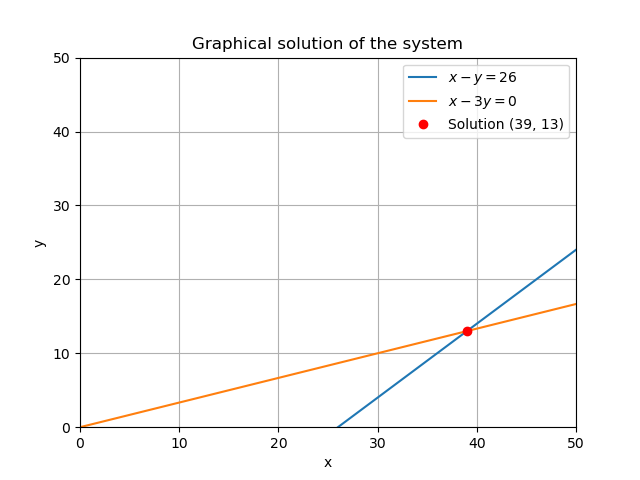
\includegraphics[width=0.6\columnwidth]{Figs/Fig1.png}
\end{center}
\caption{}
\label{fig:Fig.1}
\end{figure}

\end{document}
